\documentclass{article}
\usepackage[utf8]{inputenc}
\usepackage{amsmath}
\usepackage{ragged2e}
\usepackage{graphicx}
\usepackage{amssymb}

\title{Homework \#7 - MAT 2250}
\author{Aden Letchworth}
\date{December 2022}

\begin{document}

\maketitle

\section*{Chapter 4.4}

\begin{gather*}\tag{\textbf{5}}
    y''(\theta) + 3y'(\theta)-y(\theta)=sec\theta \\
\end{gather*}
\begin{center}
    Since the given equation has $sec\theta$ we cannot use the method of undetermined coefficients to find a particular solution. This is because when we take the derivative of the trial solution, $ 
    sec \theta $, it becomes to messy to obtain a true solution.\\
\end{center}
\begin{gather*}\tag{\textbf{15}}
    \frac{d^2y}{dx^2}-5\frac{dy}{dx}+6y=xe^x\\\\
    r^2-5r+6=0\\
    r = 3, \hspace{.1cm}r = 2\\
    y_h = c_1e^{3t}+c_2e^{2t}\\
    y_p = (Ax+B)e^x\\
    y'p = (Ax+B+A)e^x\\
    y''_p = (Ax+B+2A)e^x\\
    (Ax+B+2A)e^x-5((Ax+B+A)e^x)+6((Ax+B)e^x) = xe^x\\
    Axe^x+Be^x+2Ae^x-5Axe^x-5Be^x-5Ae^x+6Axe^x+6Be^x = xe^x\\
    2Axe^x+2Be^x-3Ae^x=xe^x\\
    2A=1,\; 2B-3A=0\\
    A = \frac{1}{2},\hspace{.2cm} B = \frac{3}{4}\\
    y_p = \frac{x}{2}e^x+\frac{3}{4}e^x\\\\
    y = c_1e^{3t}+c_2e^{2t} + \frac{x}{2}e^x+\frac{3}{4}e^x
\end{gather*}
\newpage
\begin{gather*}\tag{\textbf{28}}
    y''-6y'+9y = 5t^6e^{3t}\\\\
    r^2-6r+9 = 0\\
    r = 3\\
    y(p) = (A_6t^6+A_5t^5+A_4t^4+A_3t^3+A_2t^2+A^1t+A_0)e^{3t}
\end{gather*}
\section*{Chapter 4.5}
    \begin{gather*}\tag{\textbf{5}}
        \theta''-\theta'-2\theta=1-2t,\hspace{.5cm}\theta_p(t) = t-1\\\\
        r^2 - r - 2 = 0\\
        r = 2, \hspace{.2cm}r = -1\\
        \theta_h = c_1e^{2r}+c_2e^{-t}\\\\
        \theta_g = c_1e^{2r}+c_2e^{-t} + t - 1\\\\\\\\\\
        \tag{\textbf{32}}
        y''-y=e^{2t}+te^{2t}+t^2e^{2t}\\\\
        r^2-1=0\\
        r = 1, \hspace{.2cm}r = -1\\
        y_h = c_1e^t+c_2e^{-t}\\
        y_p = t^0(At^2+Bt+C)e^{2t}\\
        y'_p = (2At+B)e^{2t}+2(Aat^2+Bt+C)e^{2t}\\
        y'_p = (2At^2+(2A+2B)t+2C)e^{2t}\\
        y''_p = (4At+2A+2B)e^{2t} + (4At^2+(4A+4B)t+4C)e^{2t}\\
        y''_p = (4At^2+(8A+4B)t+(2A+2B+4C)e^{2t}\\
        (4At^2+(8A+4B)t+(2A+2B+4C)e^{2t} - (At^2+Bt+C)e^{2t} = e^{2t}+te^{2t}+t^2e^{2t}\\
        (3At^2+(8A+3B)t+(2A+2B+3C))e^{2t} = e^{2t}+te^{2t}+t^2e^{2t}\\
        3A = 1, \hspace{.2cm}8A+3B = 1,\hspace{.2cm}2A+2B+3C=1
        A = \frac{1}{3}, \hspace{.2cm}B = -\frac{5}{9},\hspace{.2cm}C = \frac{13}{27}\\\\
        y_p = \left(\frac{1}{3}t^2-\frac{5}{9}t+\frac{13}{27}\right)e^{2t}\\
    \end{gather*}
    \newpage
    \section{Chapter 4.9}
    \begin{center}
        The motion of a mass spring system with damping is governed by
        \RaggedLeft{(\textbf{6})}
    \end{center}
    \begin{gather*}
        y''(t)+4y'(t)+ky(t)=0;\\
        y(0) = 1, \hspace{.5cm}y'(0) = 0\\
    \end{gather*}
    \begin{center}
        Find the equation of motion and sketch its graph for k = 2, 4, and 6.
    \end{center}
    \begin{gather*}
        \\
        r^2+4r+k=0\\
        r= 2 + \sqrt{4-k}, \hspace{.5cm}2 - \sqrt{4-k}\\
    \end{gather*}
    \begin{center}
        When $k < 4$ we have two distinct roots, if $k = 4$ we have a double root,if $k > 4$ we have two complex conjugate roots
    \end{center}
    \begin{gather*}
        k = 2 \implies r= 2 + \sqrt{4-2}, \hspace{.5cm}2 - \sqrt{4-2}\\
        y(t) = Ae^{(2+\sqrt{2})t} + Be^{(2-\sqrt{2})t}\\
        1 = Ae^{(2+\sqrt{2})0} + Be^{(2-\sqrt{2})0}
        1 = A + B\\
        y'(t) = (2+\sqrt{2})Ae^{(2+\sqrt{2}t)}+(2-\sqrt{2})Be^{(2-\sqrt{2})t}\\
        0 = (2+\sqrt{2})Ae^{(2+\sqrt{2}0)}+(2-\sqrt{2})Be^{(2-\sqrt{2})0}\\
        (2+\sqrt{2})A + (2-\sqrt{2})B = 0\\
        A = \frac{1-\sqrt{2}}{2},\hspace{.5cm} B = \frac{1+\sqrt{2}}{2}\\
        y(t) = \frac{1-\sqrt{2}}{2}e^{(2+\sqrt{2})t}+ \frac{1+\sqrt{2}}{2}e^{(2-\sqrt{2})t}\\\\\\\\
        k = 4 \implies r= 2 + \sqrt{4-4}, \hspace{.5cm}2 - \sqrt{4-4}\\
        y(t) = Ae^{2t}+Bte^{2t}\\
        1 = Ae^{2(0)}+B(0)e^2{0}\\
        1 = A\\
        y'(t) = 2Ae^{2t}+(1+2t)Be^{2t}\\
        0 = 2Ae^{2(0)}+(1+2(0))Be^{2t}
        0 = 2A + B\\
        A = 1,\hspace{.5cm}B = -2\\
        y(t) = e^{2t}-2te^{2t}\\\\\\\\
        k = 6 \implies r= 2 + \sqrt{4-6}, \hspace{.5cm}2 - \sqrt{4-6}\\
        y(t) = Ae^{2t}\cos(\sqrt{2}t)+Be^{2t}\sin(\sqrt{2}t)\\
        1 = Ae^{2(0)}\cos(\sqrt{2}(0))+Be^{2(0)}\sin(\sqrt{2}(0))\\
        1 = A \\
        y'(t) = Ae^{2t}(2\cos(\sqrt{2}t)-\sqrt{5}\sin(\sqrt{2}t))+Be^{2t}(2\sin(\sqrt{2}t)+\sqrt{2}\cos(\sqrt{2}t))\\
        0 = Ae^{2(0)}(2\cos(\sqrt{2}(0))-\sqrt{5}\sin(\sqrt{2}(0))+Be^{2(0)}(2\sin(\sqrt{2}(0))+\sqrt{2}\cos(\sqrt{2}(0)))\\
        2A+\sqrt{2}B = 0\\
        A = 1, \hspace{.5cm}B = -\sqrt{2}\\
        y(t) = e^{2t}\cos(\sqrt{2}t)-\sqrt{2}e^{2t}\sin(\sqrt{2}t)\\
    \end{gather*}
    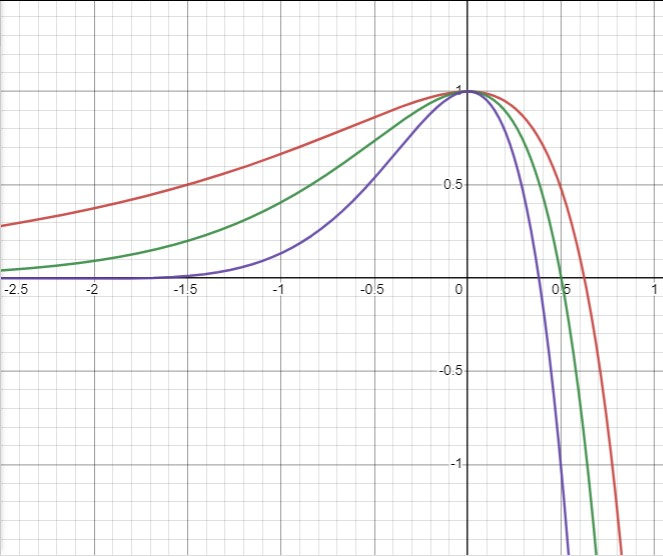
\includegraphics[width=125mm]{Screenshot 2022-12-05 165503.jpg}
    \section*{Chapter 6.1}
    \begin{gather*}\tag{\textbf{8}}
        \{x^2,x^2-1,5\} \text{ on } (-\infty,\infty)\\\\
        W(x^2,x^2-1,5) = 
        \begin{vmatrix}
            x^2 & x^2-1 & 5\\
            2x & 2x & 0\\
            2 & 2 & 0
        \end{vmatrix}\\\\
        W(x^2,x^2-1,5) =  5(2(2x)-(2x)2)\\
        W(x^2,x^2-1,5) = 0\\
    \end{gather*}
    \begin{center}
        since the Wronskian of our functions is zero we can say our functions are linearly dependent on the interval $(-\infty,\infty)$
    \end{center}
    \begin{gather*}
        y'''+2y''-11y-12y=0;\\
        \{e^{3x},e^{-x},e^{-4x}\}\\\\
        W(e^{3x},e^{-x},e^{-4x}) =
        \begin{vmatrix}
            e^{3x} & e^{-x} & e^{-4x}\\
            3e^{3x} & -e^{-x} & -4e^{-4x}\\
            9e^{3x} &  e^{-x} & 16e^{-4x}
        \end{vmatrix}
        \\\\
        W(e^{3x},e^{-x},e^{-4x}) = (e^{3x})(-e^{x}(16e^{-4x} - (-4e^{-4x})e^{-x})\\ -3e^{3x}(e^{-x}(16e^{-4x})-e^{-4x}(e^{-x})\\ +  9e^{3x}(e^{-x}(-4e^{-4x}) - e^{-4x}(-e^{-x}))\\
        W(e^{3x},e^{-x},e^{-4x}) = -4e^{-2x}(16e^{8x}+5)
    \end{gather*}
    \begin{center}
        We can say the given functions are linearly independent for $\mathbb{R}$ and therefore form a fundamental set of solutions. We know the general solution is a linear combination of our fundamental solution set of solutions.
    \end{center}
    \begin{gather*}
        y(x) = C_1e^{3x}+C_2e^{-x}+C_3e^{-4x}
    \end{gather*}
    \begin{gather*}\tag{\textbf{6}}
        x'_1 = (\cos2t)x_1\\
        x'_2 = (\sin2t)x_2\\
        x'_3 = x_1-x_2\\
        x' =
        \begin{bmatrix}
            x_1\\x_2\\x_3
        \end{bmatrix}'
        = 
        \begin{bmatrix}
            \cos(2t) & 0 & 0\\
            0 & \sin(2t) & 0\\
            1 & -2 & 0
        \end{bmatrix}
        \begin{bmatrix}
            x_1 \\ x_2 \\ x_3
        \end{bmatrix}
        \\\\\\\\
        x'' + 3x + 2y = 0 \tag{\textbf{11}}\\
        y'' - 2x = 0\\\\
        x_1 = x,\;x_2 = x',\;x_3 = y,\;x_4 = y'\\
        \begin{bmatrix}
            x_1\\x_2\\x_3\\x_4
        \end{bmatrix}'
        =
        \begin{bmatrix}
            0 & 1 & 0 & 0\\
            -3 & 0 & -2& 0\\
            0 & 0 & 0 & 1\\
            2 & 0 & 0 & 0
        \end{bmatrix}
        \begin{bmatrix}
            x_1 \\ x_2 \\ x_3 \\ x_4
        \end{bmatrix}
    \end{gather*}
\end{document}

